%tag:000X
%label:"con:symplecticCohomologyLimit"
%author:JeffHicks
%name:"$\SH(X)$ as a limit"
%type:"construction"


    As before, let $(X, \lambda)$ be a Liouville domain. For $m\not\in \ell(\Gamma)$ not a period of a Reeb orbit, define 
    \[\SH(X)^{< m}:=\HF(\hat X, H^m_t)\]
    where $H^m_t$ is a Hamiltonian which on the symplectization agrees with $H^m$, the linear Hamiltonian of slope $m$. 
    Over the symplectization $\RR\times \partial X$ there are no Hamiltonian orbits, as $H^m$ has no Hamiltonian orbits. The $< m$ signifies that this version of symplectic cohomology is only supposed to detect those Reeb orbits of period less than $m$.

    In order to recover the symplectic cohomology, we would like to understand the limit of the groups $SH(X)^{< m}$ as we take $m\to\infty$. Making sense of a limit algebraically requires constructing maps between these groups. When $m^+< m^-$, the maximum principle arguments applied to families of Hamiltonians dependent on the $s$-parameter hold, allowing us to construct chain maps 
    \[\CF(\hat X, H^{m^+}_t)\to \CF(\hat X, H^{m^-}_t)\]
    The $\pm$ index on the slope are meant to represent whether they are the incoming or outgoing side of a Floer trajectory, not the relative sizes of the slopes. From the perspective of \cref{con:symplecticCohomologyQuadratic}, the set of Hamiltonian orbits corresponding to Reeb orbits of period less than $m^+$ is a subcomplex of the set of Reeb orbits of period less than $m^-$. Intuitively, the Floer trajectory should decrease the action associated to the Reeb vector field, which is the period of the Reeb orbit.
    %label:"fig:limitHamiltonian"
%author:JeffHicks
%name:"limit Hamiltonian"
%type:"figure"
%parent:"con:symplecticCohomologyLimit"
%caption:"A limit of Hamiltonians of increasing slopes eventually sees all Reeb orbits"

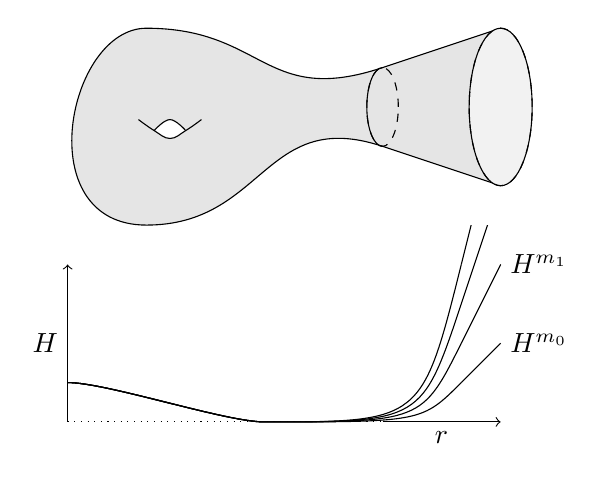
\begin{tikzpicture}
    \draw[fill=gray!20] (4,-0.5) .. controls (2.5,-1) and (4,-0.5) .. (2.5,-1) .. controls (1,-1.5) and (1,-0.5) .. (-0.5,-0.5) .. controls (-1.5,-0.5) and (-2,-3) .. (-0.5,-3) .. controls (1,-3) and (1,-1.5) .. (2.5,-2) .. controls (4,-2.5) and (2.5,-2) .. (4,-2.5);
    \begin{scope}[shift={(3.2,-2)}]
    
    \fill[white]  plot[smooth, tension=0.7] coordinates { (-3.6,0.2) (-3.4,0.1) (-3.2,0.2) }  plot[smooth, tension=0.7] coordinates {(-3.6,0.2) (-3.4,0.34) (-3.2,0.2)};
    
    \draw  plot[smooth, tension=0.7] coordinates {(-3.8,0.34) (-3.6,0.2) (-3.4,0.1) (-3.2,0.2) (-3,0.34)};
    \draw  plot[smooth, tension=0.7] coordinates {(-3.6,0.2) (-3.4,0.34) (-3.2,0.2)};
    
    
    
    \end{scope}
    
    \begin{scope}[]
    
    \draw[dashed]  (2.5,-1.5) ellipse (0.2 and 0.5);
    \clip  (2,-1) rectangle (2.5,-2);
    
    \draw  (2.5,-1.5) ellipse (0.2 and 0.5);
    \end{scope}
    
    \begin{scope}[scale=2, shift={(-0.5,0.75)}]
    
    \draw[dashed, fill=gray!10]  (2.5,-1.5) ellipse (0.2 and 0.5);
    
    
    \draw  (2.5,-1.5) ellipse (0.2 and 0.5);
    \end{scope}
    \clip  (5,-6) rectangle (-2,-3);
    \draw[dotted] (-1.5,-5.5) -- (2.5,-5.5);
    \draw[->] (2.5,-5.5) --node[below]{$r$} (4,-5.5);
    \draw (-1.5,-5) .. controls (-1,-5) and (0.5,-5.5) .. (1,-5.5) .. controls (3,-5.5) and (3,-5.5) .. (3.5,-5);
    \draw (-1.5,-5) .. controls (-1,-5) and (0.5,-5.5) .. (1,-5.5) .. controls (3,-5.5) and (3,-5.5) .. (3.5,-3.5);
    \draw (-1.5,-5) .. controls (-1,-5) and (0.5,-5.5) .. (1,-5.5) .. controls (3,-5.5) and (3,-5.5) .. (3.5,-4);
    \draw (-1.5,-5) .. controls (-1,-5) and (0.5,-5.5) .. (1,-5.5) .. controls (3,-5.5) and (3,-5.5) .. (3.5,-4.5);
    
    \draw[->] (-1.5,-5.5) -- node[left]{$H$} (-1.5,-3.5);
    \draw (3.5,-5) -- (4,-4.5) (3.5,-4.5) -- (4,-3.5) (3.5,-4) -- (4,-2.5) (3.5,-3.5) -- (4,-1.5);
    
    \node[right] at (4,-4.5) {$H^{m_0}$};
    \node[right] at (4,-3.5) {$H^{m_1}$};
    \node[right] at (4,-2.5) {$\vdots$};
    \end{tikzpicture}

    Consider now an increasing sequence of slopes $m_0< m_1< \cdots $ which are not the periods of any Reeb orbits of $\partial X$. One can form the telescope complex
    %label:"dig:symplecticCohomologyTelescope"
%type:"diagram"
%parent:"con:symplecticCohomologyLimit"
%author:JeffHicks

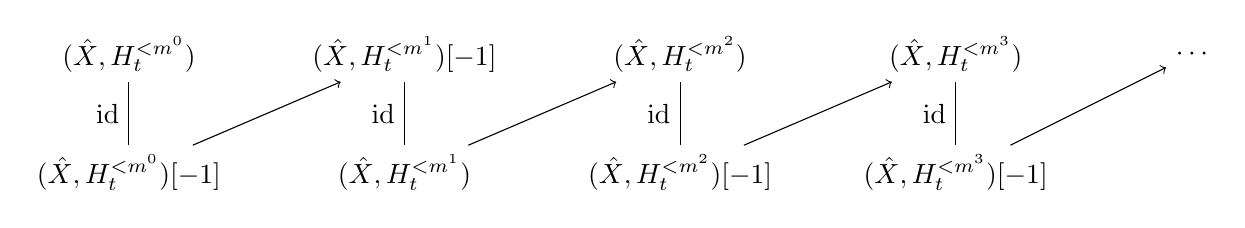
\begin{tikzpicture}
    \node (v1) at (-15,-2.5) {$\CF(\hat X, H_t^{<m^0})[-1]$};
    \node (v2) at (-15,-1) {$\CF(\hat X, H_t^{<m^0})$};
    \node (v4) at (-11.5,-1) {$\CF(\hat X, H_t^{<m^1})[-1]$};
    \node (v3) at (-11.5,-2.5) {$\CF(\hat X, H_t^{<m^1})$};
    \node (v5) at (-8,-2.5) {$\CF(\hat X, H_t^{<m^2})[-1]$};
    \node (v6) at (-8,-1) {$\CF(\hat X, H_t^{<m^2})$};
    \node (v8) at (-4.5,-1) {$\CF(\hat X, H_t^{<m^3})$};
    \node (v7) at (-4.5,-2.5) {$\CF(\hat X, H_t^{<m^3})[-1]$};
    \node (v9) at (-1.5,-1) {$\cdots$};
    \draw  (v1) edge node[left]{id} (v2);
    \draw  (v3) edge node[left]{id}  (v4);
    \draw  (v5) edge node[left]{id} (v6);
    \draw  (v7) edge node[left]{id}  (v8);
    \draw  (v1) edge[->] (v4);
    \draw  (v3) edge[->] (v6);
    \draw  (v5) edge[->] (v8);
    \draw (v7) edge[->] (v9);
\end{tikzpicture}
    where the vertical maps are the identity, and the diagonal maps are continuations.
    %label:"prp:homologyOfTelescope"
%author:JeffHicks
%name:"homology of telescope complex"
%type:"proposition"


    The cohomology of the telescope complex $\bigoplus_{i=0}^\infty C^\bullet_i \oplus C^\bullet_{i-1}$ is $\lim_{i\to\infty} H(C^\bullet_i)$.
 
    We could therefore also define
    \[SH(X):=\lim_{i\to\infty} \SH(X)^{< m^i}.\]
